\subsection{Parametric sensitivity analysis}\label{sec:sensitivity_study}
\noindent This section performs a parametric sensitivity study on the reference tracking performance of \ac{DeePC}, \ac{CL-DeePC}, and the oracle. %, thereby providing contribution~5. %
Investigated parameters are the number of past data points $\bar{N}$, the innovation noise variance $\Sigma(e_k)$, and the window lengths $p=f$. As a measure of the reference tracking performance a scaled root mean square of the reference tracking error is used: $J_\mathrm{rms}=\sqrt{\big(\sum_k r_k^2\big)\inv\sum_k(y_k-r_k)^2}$. %, scaled by the root mean square of the reference signal, is used. %
To reflect purely the effect on performance during adaptive closed-loop operation, the first $\bar{N}$ control actions are excluded. Note that it is possible for \ac{DeePC} and \ac{CL-DeePC} to outperform the oracle because the oracle does also not account for noise.

\subsubsection{Number of past data samples: $\bar{N}$}
\noindent The effect of a varying number of past data samples $\bar{N}$ is shown in Fig.~\ref{fig:varying_Nbar}. Slight fluctuations of the displayed oracle performance are an artifact that is attributable to the exclusion of the first $\bar{N}$ control actions in the calculation of $J_\mathrm{rms}$ to exclude control actions that are based on open-loop data. Using \ac{CL-DeePC} the reference tracking performance approaches the oracle's performance at a relatively low $\bar{N}$. For \ac{DeePC} the picture is different, with the median reference tracking performance remaining $26\%$ higher than its oracle counterpart at $\bar{N}=1039$. By comparison this value is only $4\%$ for \ac{CL-DeePC}.
% ------------------------- Figure --------------------------
\begin{figure}[t!]
\begin{center}
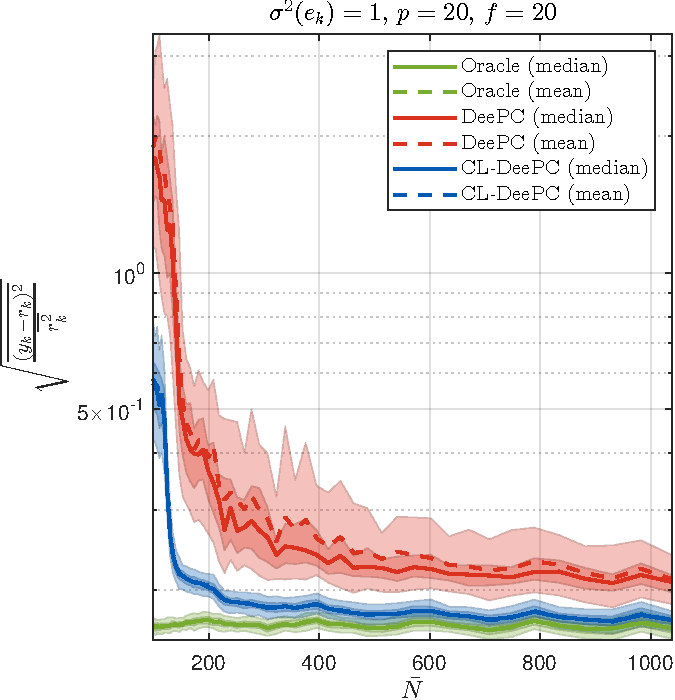
\includegraphics[width=\columnwidth]{results/figures/Varying_Nbar_99-1039-50_p_20_f_20_Re_1_Ru_1_Rdu_0_Q_100_R_0_dR_10.pdf}    % The printed column  
\caption{Effect of $\bar{N}$ on reference tracking performance. Shaded regions indicate the 10\textsuperscript{th}, 30\textsuperscript{th}, 70\textsuperscript{th} and 90\textsuperscript{th} percentiles of 120 simulations.\\}  % width is 8.4 cm.
\label{fig:varying_Nbar}                                 % Size the figures 
\end{center}                                 % accordingly.
\end{figure}
% -----------------------------------------------------------

Fig.~\ref{fig:varying_Nbar} demonstrates that compared to \ac{DeePC}, in general \ac{CL-DeePC} is able to use fewer past data samples to obtain as good or better performance, hence refered to as better sample efficiency. Compared to \ac{DeePC}, the better sample efficiency of \ac{CL-DeePC} is attributable to the use of a shorter future prediction window length for identification ($f_\mathrm{ID}=1$ as opposed to $f_\mathrm{ID}=f$). This leaves more columns $N=\bar{N}-p-f_\mathrm{ID}+1$ to approximate the relevant correlation matrices that are used implicitly by both \ac{DeePC} and \ac{CL-DeePC}. In addition, the discussed closed-loop identification issue entails that even if $\bar{N}$, and therefore $N$, is large such that these correlation matrices are approximated well, \ac{CL-DeePC} outperforms \ac{DeePC}.

\subsubsection{Noise level: $\Sigma(e_k)$}
\noindent The effect of the noise level, as quantified by a varying innovation noise variance $\Sigma(e_k)$, is shown in Fig.~\ref{fig:varying_Re}. In the absence of noise, \ac{DeePC} and \ac{MPC} are equivalent~\citep{Coulson2019}. In the noiseless case, the closed-loop identification issue does not arise so the performance of the three algorithms is identical. As the noise level increases, correlation between inputs and preceding noise increases because $|e_k|$ is typically larger, and more control effort is needed to perform noise rejection. Consequently, the closed-loop identification issue becomes more troublesome for \ac{DeePC} at higher noise levels. Note that the performance of all methods decreases with an increasing noise level because all methods lack the ability to immediately compensate noise disturbances. Using the slopes of the median performance as a measure for the susceptibility to noise-induced performance deterioration, \ac{CL-DeePC} is 48\% less susceptible to noise-induced performance deterioration compared to \ac{DeePC}.%The mean slopes of the median performance over the complete range of shown noise levels are 0.0762, 0.0958, and 0.1848 for respectively the oracle, \ac{CL-DeePC}, and \ac{DeePC}. Using this as a measure for the susceptibility to noise, these slopes indicate that, e.g., the reference tracking performance of \ac{CL-DeePC} is 48\% less susceptible to noise-induced deterioration compared to \ac{DeePC}.
% ------------------------- Figure --------------------------
\begin{figure}[t!]
\begin{center}
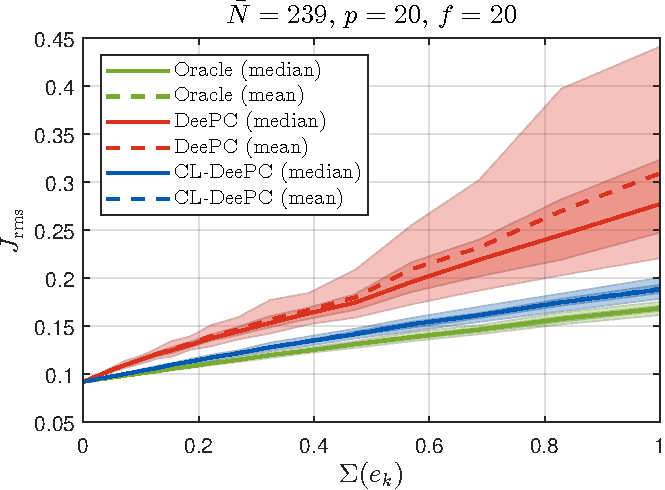
\includegraphics[width=\columnwidth]{results/figures/Varying_Re_0.0001-1-50_Nbar_239_p_20_f_20_Ru_1_Rdu_0_Q_100_R_0_dR_10.pdf}    % The printed column 
\caption{Effect of $\Sigma(e_k)$ on reference tracking performance. Shaded regions indicate the 10\textsuperscript{th}, 30\textsuperscript{th}, 70\textsuperscript{th} and 90\textsuperscript{th} percentiles over 120 simulations.}  % width is 8.4 cm.
\label{fig:varying_Re}                                 % Size the figures 
\end{center}                                 % accordingly.
\end{figure}
% -----------------------------------------------------------

\subsubsection{Data window lengths: $p=f$}
% ------------------------- Figure --------------------------
\begin{figure}[t!]
\begin{center}
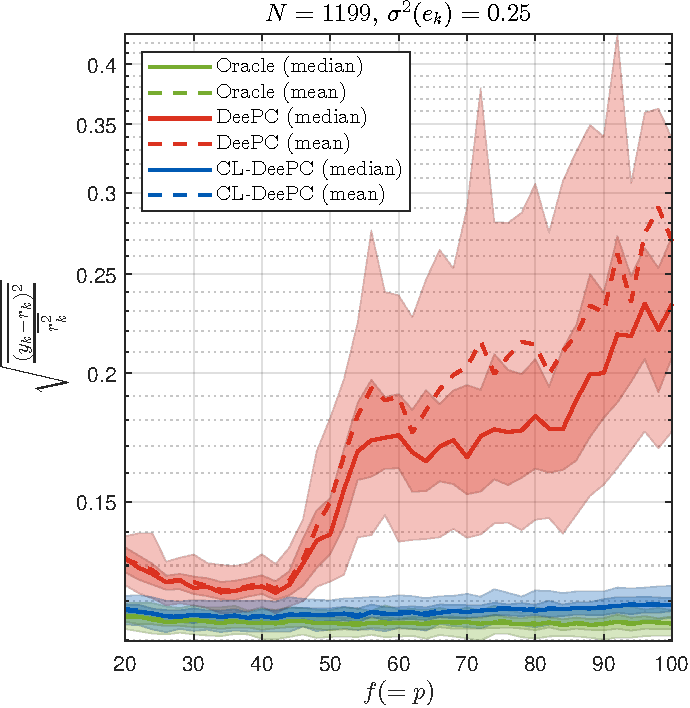
\includegraphics[width=\columnwidth]{results/figures/Varying_pf_20-100-41_Nbar_1199_Re_0.25_Ru_1_Rdu_0_Q_100_R_0_dR_10.pdf}    % The printed column 
\caption{Effect of $f=p$ on reference tracking performance. Shaded regions indicate the 10\textsuperscript{th}, 30\textsuperscript{th}, 70\textsuperscript{th} and 90\textsuperscript{th} percentiles of 120 simulations.}  % width is 8.4 cm.
\label{fig:varying_pf}                                 % Size the figures 
\end{center}                                 % accordingly.
\end{figure}
% -----------------------------------------------------------
\noindent This section investigates the effect of the window lengths with $p=f$. The choice $p=f$ is made for the sake of simplicity is further motivated by its frequent use in the closely related field of subspace identification~\citep{vanderVeen2013}. We discern two competing mechanisms to explain the results shown in Fig.~\ref{fig:varying_pf} for \ac{CL-DeePC} and an additional detrimental effect on performance for \ac{DeePC}. Increasing $p$ is beneficial in terms of reducing the bias of the predictor. However, as with increasing $f_\mathrm{ID}$, increasing $p$ entails implicitly estimating more parameters of the predictor, thereby increasing its variance. This is more pronounced for \ac{DeePC} since $f_\mathrm{ID}=f$ when compared to \ac{CL-DeePC} for which $f_\mathrm{ID}=1$. The shorter future window length used for identification $f_\mathrm{ID}$ is also beneficial for \ac{CL-DeePC} because a higher degree of collinearity may be expected for larger $f_\mathrm{ID}$, potentially leading to ill-conditioning of the identification task~\citep{Chiuso2004}. Together with the aforementioned closed-loop identification issue these effects induce up to a 49\% lower reference tracking cost at $p=f=100$ for \ac{CL-DeePC} compared to \ac{DeePC}. Moreover, note that the performance of \ac{DeePC} deteriorates rapidly with increasing $p=f$, whereas the impact on the performance of \ac{CL-DeePC} is far less pronounced.
% 1) period of 200 time samples\\
% 2) increase p -> smaller bias, but larger variance (increase number of estimated parameters)\\
% 3) increasing collinearity \& ill conditioning\\
